\documentclass[dvips, lscape]{foils}
\textwidth 18.5cm
\textheight 25cm 
\topmargin -1cm 
\oddsidemargin  -1cm 
\evensidemargin  -1cm

% Maths
\usepackage{amsfonts, amsmath, amssymb}

\newcommand{\coefbin}[2]{\left( 
    \begin{array}{c} #1 \\ #2 \end{array} 
  \right)}
\newcommand{\Bcal}{\mathcal{B}}
\newcommand{\Ccal}{\mathcal{C}}
\newcommand{\Dcal}{\mathcal{D}}
\newcommand{\Ecal}{\mathcal{E}}
\newcommand{\Gcal}{\mathcal{G}}
\newcommand{\Mcal}{\mathcal{M}}
\newcommand{\Ncal}{\mathcal{N}}
\newcommand{\Pcal}{\mathcal{P}}
\newcommand{\Qcal}{\mathcal{Q}}
\newcommand{\Lcal}{\mathcal{L}}
\newcommand{\Tcal}{\mathcal{T}}
\newcommand{\Ucal}{\mathcal{U}}
\newcommand{\alphabf}{\mbox{\mathversion{bold}{$\alpha$}}}
\newcommand{\betabf}{\mbox{\mathversion{bold}{$\beta$}}}
\newcommand{\gammabf}{\mbox{\mathversion{bold}{$\gamma$}}}
\newcommand{\mubf}{\mbox{\mathversion{bold}{$\mu$}}}
\newcommand{\Pibf}{\mbox{\mathversion{bold}{$\Pi$}}}
\newcommand{\psibf}{\mbox{\mathversion{bold}{$\psi$}}}
\newcommand{\thetabf}{\mbox{\mathversion{bold}{$\theta$}}}
\newcommand{\taubf}{\mbox{\mathversion{bold}{$\tau$}}}
\newcommand{\Cbf}{{\bf C}}
\newcommand{\Ebf}{{\bf E}}
\newcommand{\Gbf}{{\bf G}}
\newcommand{\Hbf}{{\bf H}}
\newcommand{\Ibf}{{\bf I}}
\newcommand{\mbf}{{\bf m}}
\newcommand{\Pbf}{{\bf P}}
\newcommand{\Sbf}{{\bf S}}
\newcommand{\Tbf}{{\bf T}}
\newcommand{\ubf}{{\bf u}}
\newcommand{\Ubf}{{\bf U}}
\newcommand{\vbf}{{\bf v}}
\newcommand{\Vbf}{{\bf V}}
\newcommand{\xbf}{{\bf x}}
\newcommand{\Xbf}{{\bf X}}
\newcommand{\Ybf}{{\bf Y}}
\newcommand{\Zbf}{{\bf Z}}
\newcommand{\Esp}{{\mathbb E}}
\newcommand{\Var}{{\mathbb V}}
\newcommand{\Cov}{{\mathbb C}\mbox{ov}}
\newcommand{\Ibb}{{\mathbb I}}
\newcommand{\Rbb}{\mathbb{R}}

% Couleur et graphiques
\usepackage{color}
%\usepackage{graphics}
\usepackage{epsfig} 

% Texte
\usepackage{lscape}
\usepackage{../../../../Latex/fancyheadings, rotating, enumerate}
%\usepackage[french]{babel}
\usepackage[latin1]{inputenc}
\definecolor{darkgreen}{cmyk}{0.5, 0, 0.5, 0.5}
\definecolor{orange}{cmyk}{0, 0.6, 0.8, 0}
\definecolor{jaune}{cmyk}{0, 0.5, 0.5, 0}
\newcommand{\textblue}[1]{\textcolor{blue}{#1}}
\newcommand{\textred}[1]{\textcolor{red}{#1}}
\newcommand{\textgreen}[1]{\textcolor{green}{ #1}}
\newcommand{\textlightgreen}[1]{\textcolor{green}{#1}}
%\newcommand{\textgreen}[1]{\textcolor{darkgreen}{#1}}
\newcommand{\textorange}[1]{\textcolor{orange}{#1}}
\newcommand{\textyellow}[1]{\textcolor{yellow}{#1}}
\newcommand{\refer}[2]{\textgreen{[{\sl #1, #2}]}}
\newcommand{\emphase}[1]{\textblue{#1}}

% Sections
%\newcommand{\chapter}[1]{\centerline{\LARGE \textblue{#1}}}
% \newcommand{\section}[1]{\centerline{\Large \textblue{#1}}}
% \newcommand{\subsection}[1]{\noindent{\Large \textblue{#1}}}
% \newcommand{\subsubsection}[1]{\noindent{\large \textblue{#1}}}
% \newcommand{\paragraph}[1]{\noindent {\textblue{#1}}}
% Sectionsred
\newcommand{\chapter}[1]{
  \addtocounter{chapter}{1}
  \setcounter{section}{0}
  \setcounter{subsection}{0}
%   {\centerline{\LARGE \textblue{\arabic{chapter} - #1}}}
  {\centerline{\LARGE \textblue{#1}}}
  }
\newcommand{\section}[1]{
  \addtocounter{section}{1}
  \setcounter{subsection}{0}
%   {\centerline{\Large \textblue{\arabic{chapter}.\arabic{section} - #1}}}
%   }
  {\centerline{\Large \textblue{#1}}}
  }
\newcommand{\subsection}[1]{
  \addtocounter{subsection}{1}
  {\noindent{\large \textblue{#1}}}
  }
% \newcommand{\subsection}[1]{
%   \addtocounter{subsection}{1}
%   {\noindent{\large \textblue{\arabic{chapter}.\arabic{section}.\arabic{subsection} - #1}}}
%   }
\newcommand{\paragraph}[1]{\noindent{\textblue{#1}}}

%%%%%%%%%%%%%%%%%%%%%%%%%%%%%%%%%%%%%%%%%%%%%%%%%%%%%%%%%%%%%%%%%%%%%%
%%%%%%%%%%%%%%%%%%%%%%%%%%%%%%%%%%%%%%%%%%%%%%%%%%%%%%%%%%%%%%%%%%%%%%
%%%%%%%%%%%%%%%%%%%%%%%%%%%%%%%%%%%%%%%%%%%%%%%%%%%%%%%%%%%%%%%%%%%%%%
%%%%%%%%%%%%%%%%%%%%%%%%%%%%%%%%%%%%%%%%%%%%%%%%%%%%%%%%%%%%%%%%%%%%%%
\begin{document}
%%%%%%%%%%%%%%%%%%%%%%%%%%%%%%%%%%%%%%%%%%%%%%%%%%%%%%%%%%%%%%%%%%%%%%
%%%%%%%%%%%%%%%%%%%%%%%%%%%%%%%%%%%%%%%%%%%%%%%%%%%%%%%%%%%%%%%%%%%%%%
%%%%%%%%%%%%%%%%%%%%%%%%%%%%%%%%%%%%%%%%%%%%%%%%%%%%%%%%%%%%%%%%%%%%%%
%%%%%%%%%%%%%%%%%%%%%%%%%%%%%%%%%%%%%%%%%%%%%%%%%%%%%%%%%%%%%%%%%%%%%%
\landscape
\newcounter{chapter}
\newcounter{section}
\newcounter{subsection}
\setcounter{chapter}{0}
\headrulewidth 0pt 
\pagestyle{fancy} 
\cfoot{}
\rfoot{\begin{rotate}{90}{
      \hspace{1cm} \tiny CGH analysis
      }\end{rotate}}
\rhead{\begin{rotate}{90}{
      \hspace{-.5cm} \tiny \thepage
      }\end{rotate}}

%%%%%%%%%%%%%%%%%%%%%%%%%%%%%%%%%%%%%%%%%%%%%%%%%%%%%%%%%%%%%%%%%%%%%%
%%%%%%%%%%%%%%%%%%%%%%%%%%%%%%%%%%%%%%%%%%%%%%%%%%%%%%%%%%%%%%%%%%%%%%
\begin{center}
  \textblue{\LARGE  CGH (+ ChIP) Arrays Analysis}
  
  \vspace{2cm}
  {\large E. Lebarbier, S. Robin, B. Thiam + M.-L. Martin-Magniette}

  %\vspace{1cm}
  robin@agroparistech.fr
  
  \vspace{2cm}
  {UMR AgroParisTech / INRA: Math�matique et Informatique Appliqu�es}
  
  {SSB group: genome.jouy.inra.fr/ssb/}
  
  \vspace{2cm}
  \begin{tabular}{ccccc}
    
\epsfig{file=../Figures/LogoINRA-Couleur.ps, width=5cm} &
    \hspace{.5cm} &
    
\epsfig{file=../Figures/logagroptechsolo.eps, width=7.5cm} &
    \hspace{.5cm} &
    \epsfig{file=../Figures/Logo-SSB.eps, width=5cm} \\
  \end{tabular} \\
  \bigskip

  \date{Saclay, February 2009}
\end{center}

%%%%%%%%%%%%%%%%%%%%%%%%%%%%%%%%%%%%%%%%%%%%%%%%%%%%%%%%%%%%%
%%%%%%%%%%%%%%%%%%%%%%%%%%%%%%%%%%%%%%%%%%%%%%%%%%%%%%%%%%%%%
\newpage
\chapter{CGH arrays}
%%%%%%%%%%%%%%%%%%%%%%%%%%%%%%%%%%%%%%%%%%%%%%%%%%%%%%%%%%%%%
%%%%%%%%%%%%%%%%%%%%%%%%%%%%%%%%%%%%%%%%%%%%%%%%%%%%%%%%%%%%%
\paragraph{Usual purpose}
\begin{itemize}
\item \vspace{-.75cm} Evaluate the number of copy at each locus
\item \vspace{-.75cm} Detect copy number variations (CNV)
\item \vspace{-.75cm} Detect chromosomic aberrations
\end{itemize}

\paragraph{AgriArray} \\
{\sl A complete CGH protocol will be developed in order to
  characterize maize breeding lines; this protocol, based on the
  Genoplante 57 K maize array and in a second time the results of WP1,
  will give access to \emphase{gene duplication or deletion events
    between lines}. Its utility as a global identification tool will
  also be evaluated, the genomic profiling being used as a plant
  barcode.}

\paragraph{Disparition of BioGemma} 
\begin{itemize}
\item \vspace{-.75cm} No precise biological demand anymore
\item \vspace{-.75cm} $\rightarrow$ Development of generic tools
\end{itemize}

%%%%%%%%%%%%%%%%%%%%%%%%%%%%%%%%%%%%%%%%%%%%%%%%%%%%%%%%%%%%%
\newpage
\subsection{Statistical analysis of one CGH profile}
%%%%%%%%%%%%%%%%%%%%%%%%%%%%%%%%%%%%%%%%%%%%%%%%%%%%%%%%%%%%%
$$
\begin{tabular}{cc}
  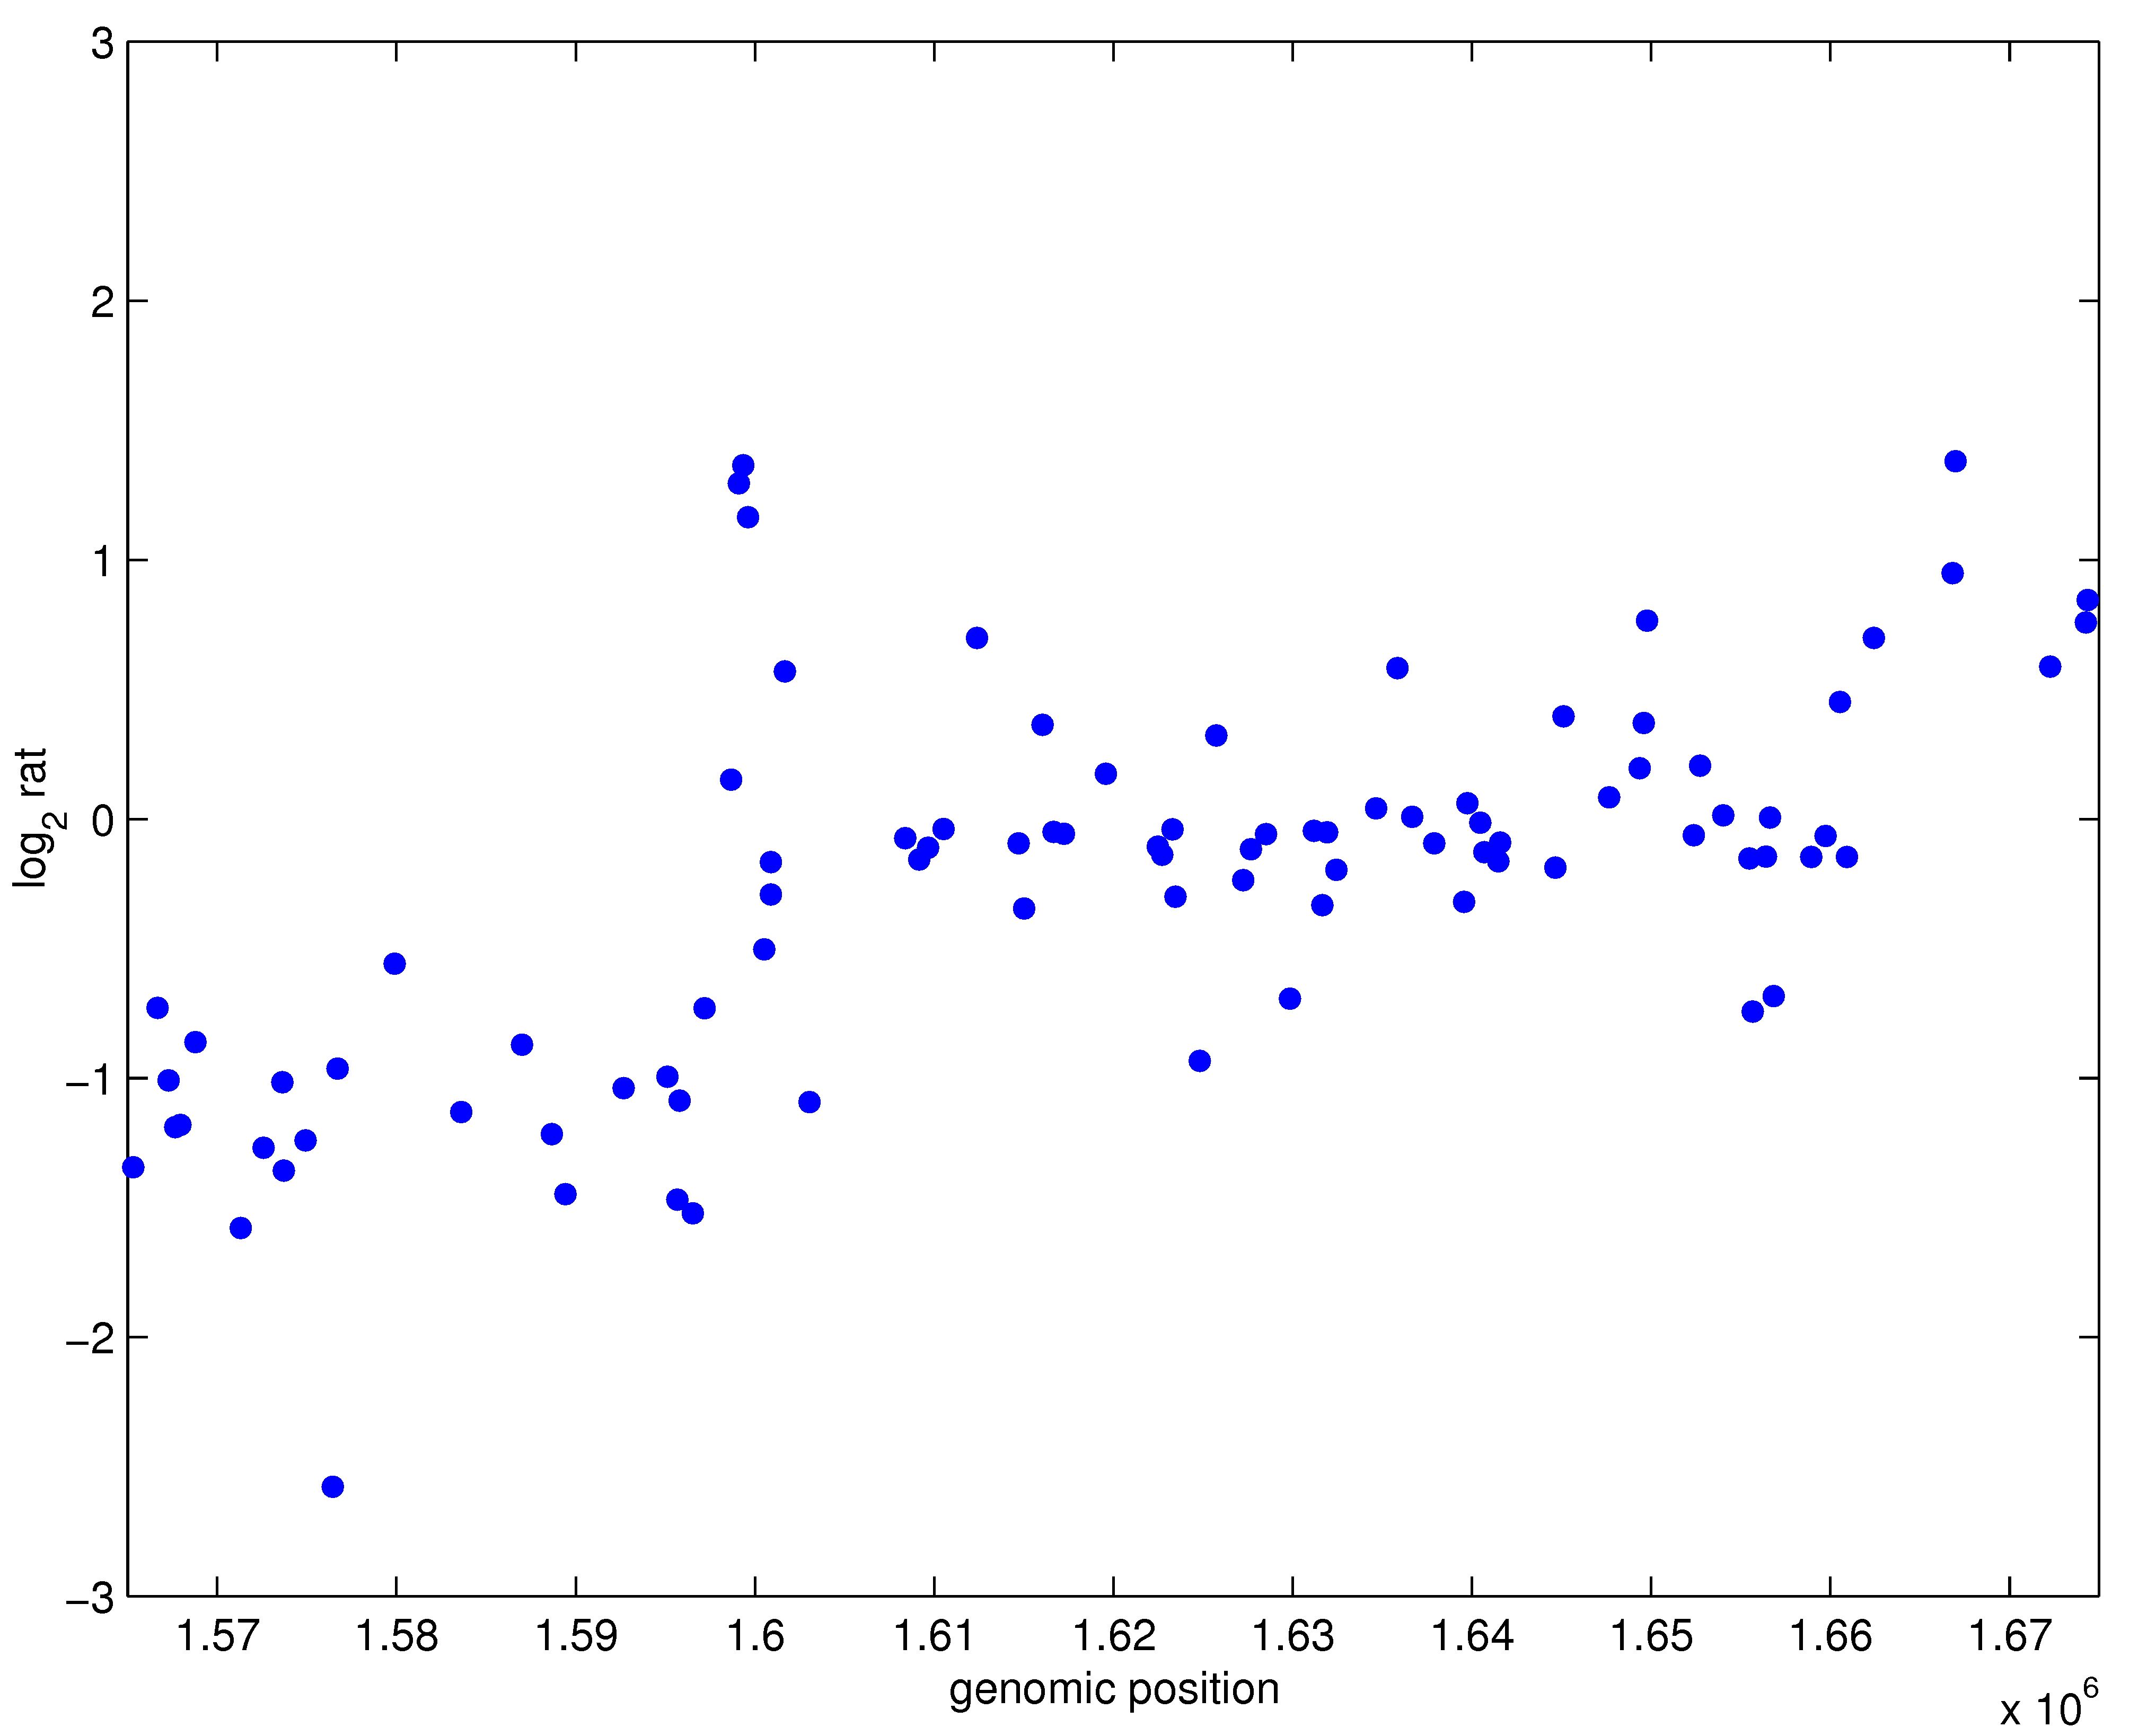
\epsfig{file = ../Figures/raw_profile_example.eps, clip=,
  width=11cm, height=11cm}
  &
  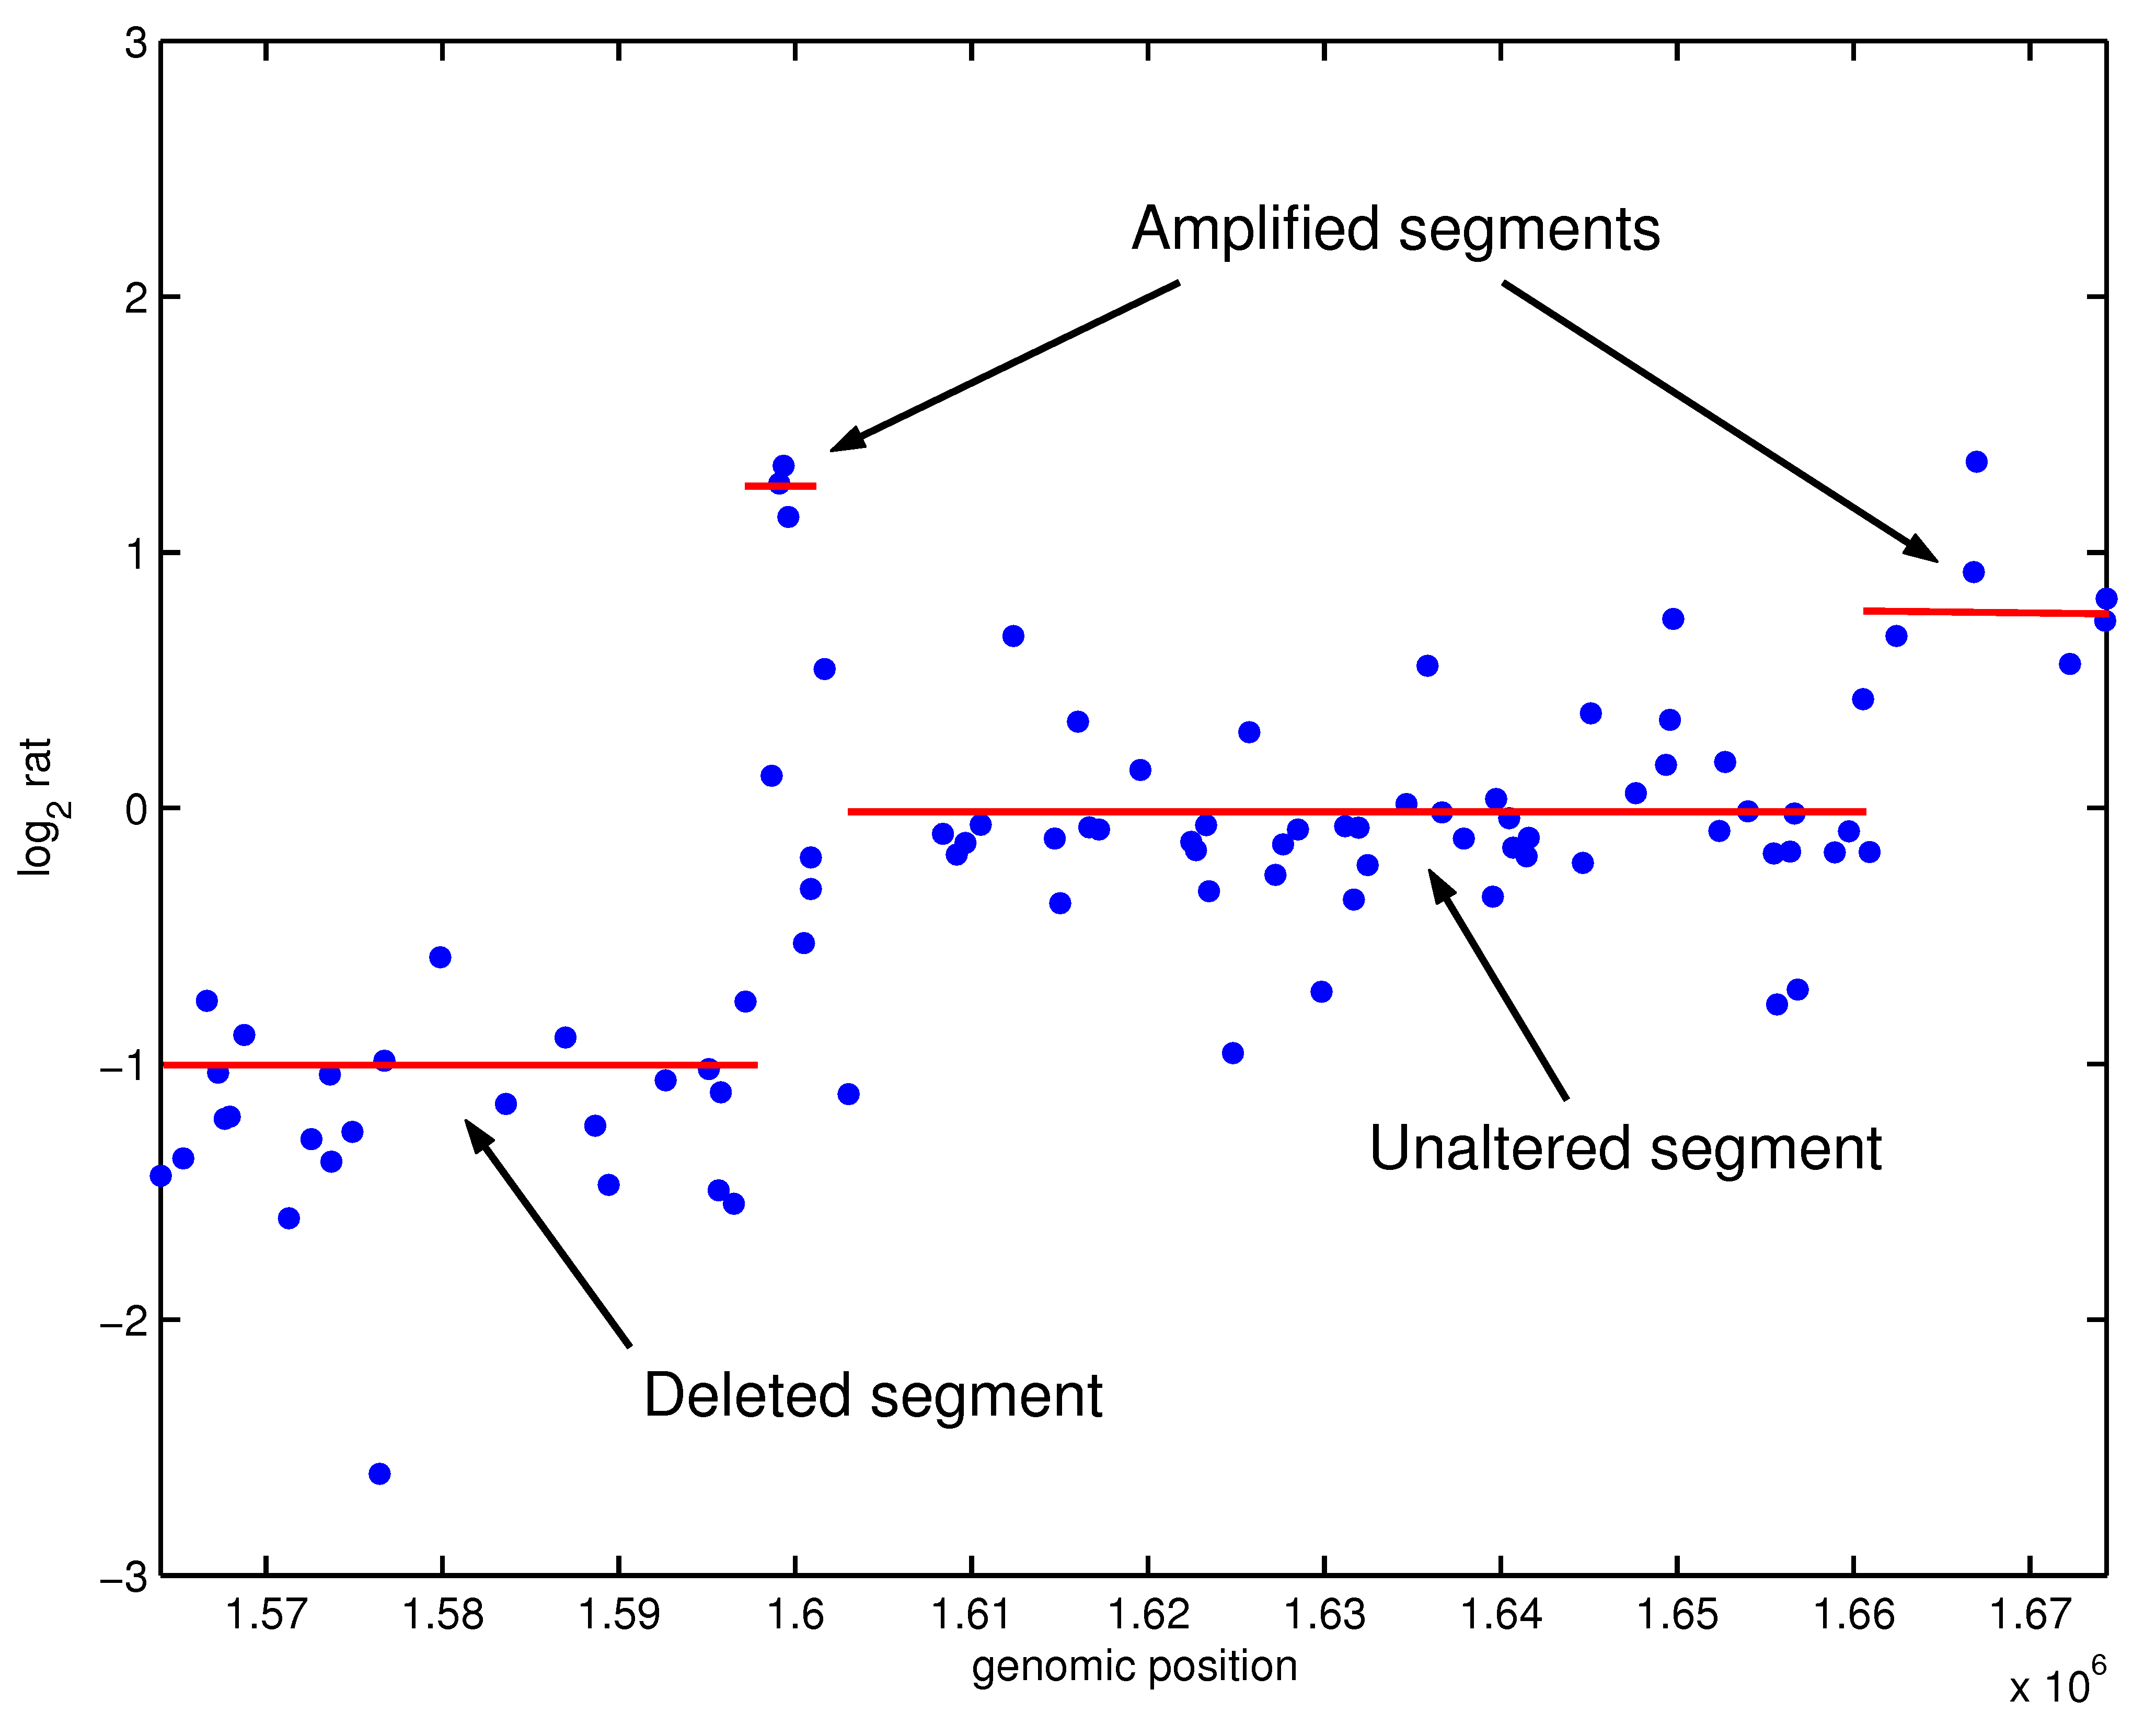
\epsfig{file = ../Figures/profile_example.eps, clip=,
    bbllx=60, bblly=196, bburx=543, bbury=586,width=11cm, height=11cm} 
\end{tabular}
$$
\begin{itemize}
\item \vspace{-.75cm} Breakpoint localisation
\item \vspace{-.75cm} Model selection
\end{itemize}

%%%%%%%%%%%%%%%%%%%%%%%%%%%%%%%%%%%%%%%%%%%%%%%%%%%%%%%%%%%%%
%%%%%%%%%%%%%%%%%%%%%%%%%%%%%%%%%%%%%%%%%%%%%%%%%%%%%%%%%%%%%
\newpage
\chapter{Mutiple array analysis}
%%%%%%%%%%%%%%%%%%%%%%%%%%%%%%%%%%%%%%%%%%%%%%%%%%%%%%%%%%%%%
%%%%%%%%%%%%%%%%%%%%%%%%%%%%%%%%%%%%%%%%%%%%%%%%%%%%%%%%%%%%%

%%%%%%%%%%%%%%%%%%%%%%%%%%%%%%%%%%%%%%%%%%%%%%%%%%%%%%%%%%%%%
\bigskip
\section{Two examples.}

\paragraph{1 - Comparing {\sl A. Thaliana} mutants or ecotypes.}
Chromosomal rearrangement can be detected by comparing CGH profiles
observed on individual from different genotypes. ({\sl Supported by
  ANR/G�noplante AgriArray project}.)

\paragraph{2 - Comparing groups of patients.}
To detect chromosomal aberration associated with a specific disease
(e.g. breast cancer), we analyse the profiles of several ill patients
jointly.

\bigskip\bigskip
\subsection{First approach: Common breakpoints.}

Assuming that all the patients of the same group have their
breakpoints at the same positions, leads to \emphase{segment a
  multivariate signal}, which can be achieved using DP.

This is doable but \emphase{biologically irrelevant}.

%%%%%%%%%%%%%%%%%%%%%%%%%%%%%%%%%%%%%%%%%%%%%%%%%%%%%%%%%%%%%
\newpage
\section{Segmentation / Regression}

\hspace{-2cm}
\begin{tabular}{cc}
  \begin{tabular}{p{12cm}}
    We want 
    \begin{itemize}
    \item to allow \emphase{profile specific
        breakpoints}, 
    \item \vspace{-.75cm} accounting for common \emphase{probe
        effect}, since \emphase{different probe affinities} may alter
      all the profiles at the same position.
    \end{itemize}

    \bigskip
    Denoting $Y_{it}$ the profile of patient $i$ at position $t$
    (belonging to segment $I_{ik}$), we
    set
    $$
    Y_{it} = \mu_{ik} + \theta_t + E_{it}
    $$
    where $\mu_{ik}$ is the mean of segment $I_{ik}$ and
    \emphase{$\theta_t$ is the (fixed) effect of probe $t$}.
%     $$
%     \{E_{it}\} \mbox{ iid } \Ncal(0, \sigma^2),  
%     \quad
%     \{U_t\} \mbox{ iid } \Ncal(0, \gamma^2).  
%     $$
  \end{tabular}
  &
  \begin{tabular}{l}
    \epsfig{file = ../Figures/nakao-mat.txt-MixSeg-V2.eps, width=11cm,
    height=14cm, bbllx=90, bblly=220, bburx=380, bbury=590, clip=}
  \end{tabular}
\end{tabular}

%%%%%%%%%%%%%%%%%%%%%%%%%%%%%%%%%%%%%%%%%%%%%%%%%%%%%%%%%%%%%
\newpage
\subsection{Post-Doc of B. Thiam}

\paragraph{Existing programs}
\begin{itemize}
\item \vspace{-.75cm} Dynamic programming (DP) for one profile
  segmentation
\item \vspace{-.75cm} Second stage of DP for multiple profile
  segmentation
\item \vspace{-.75cm} Model selection to choose the number of segments 
\end{itemize}

\paragraph{B. Thiam contribution}
\begin{itemize}
\item \vspace{-.75cm} Regression step, i.e. estimation of the probe
  effect $\thetabf$ in the model
  $$
  \Ybf = \Tbf \mubf + \Xbf \thetabf + \Ebf
  $$
\item \vspace{-.75cm} Implementation in R (available for AgriArray
  partners)
\item \vspace{-.75cm} Insertion in the segmentation / regression /
  classification alternative algorithm (see next slides).
\item \vspace{-.75cm} Analysis of few {\sl A. thaliana} ecotypes.
\end{itemize}

%%%%%%%%%%%%%%%%%%%%%%%%%%%%%%%%%%%%%%%%%%%%%%%%%%%%%%%%%%%%%
\newpage
\subsection{Segmentation / Regression / Classification}

\paragraph{Clustering segments.} In addition to 
\begin{itemize}
\item \vspace{-.75cm} breakpoint detection and 
\item \vspace{-.75cm} probe effect estimation, 
\item \vspace{-.75cm} we would like to cluster segments corresponding
  with \emphase{same status} (e.g. deleted, normal, amplified)
\end{itemize}
$$
\begin{tabular}{cc}
  Pure segmentation & Segmentation + classification \\
  \epsfig{file = ../Figures/FigSegClas-1.eps, clip=, scale=0.7} &
  \epsfig{file = ../Figures/FigSegClas-2.eps, clip=, scale=0.7} \\
\end{tabular}
$$
 
%%%%%%%%%%%%%%%%%%%%%%%%%%%%%%%%%%%%%%%%%%%%%%%%%%%%%%%%%%%%%
\newpage
\paragraph{Estimation algorithm.} Three ingredients have to combined
$$
\begin{tabular}{llcl}
  1~- & Linear regression & $\rightarrow$ & Probe effect \\
  2~- & Dynamic programming & $\rightarrow$ & Breakpoint detection \\
  3~- & Expectation-Maximisation (EM) & $\rightarrow$ & (Model-based) clustering
\end{tabular}
$$

\paragraph{Comparing strategies.} 
\begin{itemize}
\item \vspace{-.75cm} Genuine EM: segmentation within the M step
\item \vspace{-.75cm} Alternating DP (segmentation) and EM
  (regression \& classification): \\
  \begin{center}
    \vspace{-1.5cm} 
    $\rightarrow$ \emphase{no segmentation during the M step}
  \end{center}
\end{itemize}

\paragraph{Conclusions.} 
\begin{itemize}
\item \vspace{-.75cm} The genuine and alternative provide the same
  results (simulations and real data)
\item \vspace{-.75cm} The alternative strategy is much faster.
\end{itemize}


%%%%%%%%%%%%%%%%%%%%%%%%%%%%%%%%%%%%%%%%%%%%%%%%%%%%%%%%%%%%%
%%%%%%%%%%%%%%%%%%%%%%%%%%%%%%%%%%%%%%%%%%%%%%%%%%%%%%%%%%%%%
\newpage
\chapter{In progress}
%%%%%%%%%%%%%%%%%%%%%%%%%%%%%%%%%%%%%%%%%%%%%%%%%%%%%%%%%%%%%
%%%%%%%%%%%%%%%%%%%%%%%%%%%%%%%%%%%%%%%%%%%%%%%%%%%%%%%%%%%%%

%%%%%%%%%%%%%%%%%%%%%%%%%%%%%%%%%%%%%%%%%%%%%%%%%%%%%%%%%%%%%
\bigskip
\section{CGH-seg package: Generic package}
%%%%%%%%%%%%%%%%%%%%%%%%%%%%%%%%%%%%%%%%%%%%%%%%%%%%%%%%%%%%%

% \subsection{ for multiple CGH array}

\paragraph{Models and methods ({\sl with F. Picard}).}
\begin{itemize}
\item \vspace{-.75cm} Random effect model
\item \vspace{-.75cm} Segmentation / regression / classification model
  (including B. Thiam's contribution)
\item \vspace{-.75cm} Model selection criteria
\item \vspace{-.75cm} Detection of recurrent aberrations (see next
  slide)
\end{itemize}

\paragraph{Algorithms.}
\begin{itemize}
\item \vspace{-.75cm} 1- and 2-step DP algorithms for efficient
  segmentation
\item \vspace{-.75cm} Hierarchical clustering as a heuristic for very
  large signals.
\item \vspace{-.75cm} Smoothing strategy to avoid local maxima:
  improve model with $K$ segments and $P$ groups thanks to models with
  $K-1$ / $K+1$ segments or $P-1$ / $P+1$ groups
\end{itemize}

\paragraph{Outputs.}
\begin{itemize}
\item \vspace{-.75cm} Parameters estimates (breakpoint positions, ...)
\item \vspace{-.75cm} Graphical outputs
\end{itemize}

%%%%%%%%%%%%%%%%%%%%%%%%%%%%%%%%%%%%%%%%%%%%%%%%%%%%%%%%%%%%%
\newpage
\section{Detection of recurrent aberrations}
%%%%%%%%%%%%%%%%%%%%%%%%%%%%%%%%%%%%%%%%%%%%%%%%%%%%%%%%%%%%%

% \noindent
% \begin{tabular}{cc}
%   \begin{tabular}{p{7.5cm}}
%     To detect \emphase{aberrations associated to a disease}
%     (e.g. bladder cancer), we look for aberrations that appear
%     \emphase{'significantly'  often} among a set of patients.  \\ \\
%   $X_{it}$ denotes the status of position $t$ for patient $i$:
%   $$
%   \begin{tabular}{rcrl}
%     $X_{it}$ & = & \textblue{--1} & \textblue{(loss)} \\
%     & = & 0 & (normal) \\
%     & = & \textred{+1} & \textred{(gain)}
%   \end{tabular}
%   $$
%   \refer{Hupp� et al.}{2004}
%   \end{tabular}
%   &
%   \begin{tabular}{c}
%     \epsfig{file=/RECHERCHE/RUPTURES/Etudes/Curie/MinRegion/Data1/Profiles.eps,
%     }
%   \end{tabular}
% \end{tabular}

% %%%%%%%%%%%%%%%%%%%%%%%%%%%%%%%%%%%%%%%%%%%%%%%%%%%%%%%%%%%%%%%%%%%%%%
% \newpage
% \section{Minimal region}
% %%%%%%%%%%%%%%%%%%%%%%%%%%%%%%%%%%%%%%%%%%%%%%%%%%%%%%%%%%%%%%%%%%%%%%

\bigskip
\noindent
\begin{tabular}{cc}
  \begin{tabular}{p{17cm}}
    \paragraph{({\sl with V. Stefanov})} \\
    \\
    A recurrent aberration is a sequence of \emphase{successive positions}
    for which the \emphase{same status} is observed in \emphase{large
    number} of patients at the same time. \\
                                %\refer{Rouveirol \& al.}{2006}\\
    \\
    \paragraph{Data.} $M^* = 31$ patients present $\ell =
    5$ successive deletions between positions 1189 and 1193, in
    chromosome 9. \\
    \\
    \paragraph{Question.} Is this significant, given the number of
    patients ($m=84$) and the profiles length ($n=2340$)? \\
    \\
    \paragraph{'Motif statistic' problem:} How likely is it to observe
    occurrences of a same motif simultaneously in a large
    number of sequences? 
%     Source: Bladder cancer data, F. Radvanyi, C. Rouveirol, Inst. Curie
  \end{tabular}
  &
  \begin{tabular}{c}
    \epsfig{file=/RECHERCHE/RUPTURES/Etudes/Curie/MinRegion/Data1/ExMinRegion.eps,
      clip=, bbllx=270, bblly=209, bburx=400, bbury=593}
  \end{tabular}
\end{tabular}


% %%%%%%%%%%%%%%%%%%%%%%%%%%%%%%%%%%%%%%%%%%%%%%%%%%%%%%%%%%%%%%%%%%%%%%
% \newpage
% \section{Motif Statistics}
% %%%%%%%%%%%%%%%%%%%%%%%%%%%%%%%%%%%%%%%%%%%%%%%%%%%%%%%%%%%%%%%%%%%%%%

% \paragraph{Binary case.} Assume that only 2 status exist: 
% $$
% X_{it} = \left\{ 
%   \begin{array}{rl}
%     1 & \mbox{for aberration,} \\
%     0 & \mbox{for normal.}
%   \end{array}
% \right.
% $$

% \paragraph{Region.} A minimal region is then a $\ell$-run of
% 1s. Denote
% $$
% Y_{it} = \prod_{u=t-\ell+1}^t X_{it} = \left\{ 
%   \begin{array}{rl}
%     1 & \mbox{if a $\ell$-run occurs at position $t$ in profile $i$,} \\
%     0 & \mbox{otherwise.}
%   \end{array}
% \right.
% $$
% % $Y_{it} = Y_{it}(\Rcal)$ indicates the
% % occurrence of $\ell$ successive aberrations ending at position $t$ in
% % patient $i$:
% % $$
% % Y_{it}= \prod_{u=1}^{\ell} X_{i, t-u+1}.
% % $$
% \paragraph{Simultaneous occurrences.} $Y_{+t} = \sum_i Y_{it}$ is
% the number of patients for which a $\ell$ successive aberrations
% (\emphase{$\ell$-run}) occurs at $t$.

% \bigskip
% \paragraph{Significance of an observed minimal region.} We have to calculate
% $$
% \Pr\left\{\max_{\ell \leq t \leq n}Y_{+t} \geq M^*\right\}.
% $$

% %%%%%%%%%%%%%%%%%%%%%%%%%%%%%%%%%%%%%%%%%%%%%%%%%%%%%%%%%%%%%%%%%%%%%%
% \newpage
% \section{Markov Model}
% %%%%%%%%%%%%%%%%%%%%%%%%%%%%%%%%%%%%%%%%%%%%%%%%%%%%%%%%%%%%%%%%%%%%%%

% \paragraph{Model.} 
% Each profile $\{X_{it}\}_t$ is a 2-state stationary Markov chain (MC):
% $$
% \{X_{it}\}_t \sim \text{MC}(\Pibf, \mubf)
% $$
% where $\Pibf$ is the transition matrix and $\mubf$ the stationary
% distribution ($\forall i: X_{i1} \sim \mubf$).

% The patients (profiles) are supposed to be independent.

% \bigskip
% \paragraph{Estimated transition probabilities and stationary
%   distributions.} States $= \{0, 1\}$:
% $$
% \text{Gain:} \qquad\qquad
% \widehat{\Pibf}^+ = \left(\begin{array}{rr}
%        99.74 &      0.26 \\
%         1.98 &      98.02 \\
%   \end{array}\right), 
% \qquad \widehat{\mubf}^+ = (88.36 \quad      11.64), 
% $$
% $$
% \text{Loss:} \qquad\qquad
% \widehat{\Pibf}^- = \left(\begin{array}{rr}
%         99.72 &      0.28 \\
%        2.26 &       97.74 \\
%   \end{array}\right), 
% \qquad \widehat{\mubf}^- = (88.98 \quad      11.02).
% $$
% % $$
% % \widehat{\Pibf} = \left(\begin{array}{rr}
% %        99.7 & 0.3 \\
% %        2.0 &  98.0 \\
% %   \end{array}\right), 
% % \qquad \widehat{\mubf} = (88.4 \quad  11.6).
% % $$

% %%%%%%%%%%%%%%%%%%%%%%%%%%%%%%%%%%%%%%%%%%%%%%%%%%%%%%%%%%%%%%%%%%%%%%
% \newpage
% \section{Significance: One sequence}
% %%%%%%%%%%%%%%%%%%%%%%%%%%%%%%%%%%%%%%%%%%%%%%%%%%%%%%%%%%%%%%%%%%%%%%

% \paragraph{Waiting time.} What is the probability for a $\ell$-run to
% occur in a sequence with length $n$
% $$
% \Pr\left\{\max_{\ell \leq t \leq n}Y_{t} \geq 1\right\} = \Pr\{ T
% \leq n\}
% $$
% where $T$ is the waiting time befor the first occurrence of a $\ell$-run.

% \paragraph{Markov Chain embedding.} 
% We define $\{Z_t\}$, the process describing the construction of a
% $\ell$-run; $\{Z_t\}$ is a Markov chain over $\{0, \dots, \ell\}$ with
% transition matrix 
% %\vspace{-0.55cm}
% $$
% \Pbf = \left(
%   \begin{array}{c|cccccc}
%     & 0 & 1 & 2 & \dots & \ell-1 & \ell \\
%     \hline
%     0 & \pi_{00} & \pi_{01} \\
%     1 & \pi_{10} & & \pi_{11} \\
%     2 & \pi_{10} & & & \pi_{11} \\
%     \vdots & \vdots & & & & \ddots \\
%     \vdots & \pi_{10} & & & & & \pi_{11} \\
%     \ell & & & & & & 1 \\
%   \end{array}
%   \right)
% $$

% %%%%%%%%%%%%%%%%%%%%%%%%%%%%%%%%%%%%%%%%%%%%%%%%%%%%%%%%%%%%%%%%%%%%%%
% \newpage
% \paragraph{Distribution of $Z_t$.} If the profile $\{X_t\}$ starts in the
% normal state ($X_1 = 0$), we have
% $$
% \mubf_1 = [1 \;  0 \; \dots \; 0]
% $$
% the distribution of $Z_t$ is given by 
% $
% \mubf_t =  \mubf_1 \Pbf^{t-1}.
% $

% \bigskip\bigskip
% \hspace{-2cm}
% \begin{tabular}{ll}
%   \begin{tabular}{p{12cm}}
%     \paragraph{Distribution of $T$.} Noting that
%     $$
%     \Pr\{T \leq n\} = \Pr\{Z_n = \ell\}
%     $$
%     we see that the distribution of $T$ is given by the last coordinate
%     of $\mubf_n$:
%     $$
%     \Pr\{T \leq n\} = \mu_{n, \ell}.
%     $$
%     (Right panel: $\ell = 10$, $n = 1..500$) \\ \\ \\
%   \end{tabular}
%   & 
%   \begin{tabular}{p{13cm}}
%     \epsfig{file = ../FIGURES/Fig_WaitLRun.eps, width = 12cm,
%     height=10cm, clip=}
%   \end{tabular}
% \end{tabular}

% % %%%%%%%%%%%%%%%%%%%%%%%%%%%%%%%%%%%%%%%%%%%%%%%%%%%%%%%%%%%%%%%%%%%%%%
% % \newpage
% % \subsection{Remark: Markov chain embedding for other motifs}

% % Run are very particular motifs. Markov chain embedding can be used for
% % much more general motifs.

% % \paragraph{Example: Alternate losses and successes $[1 \; 0 \; 1 \;
% %   0 \; 1]$.}  
% % The $\{Z_t\}$ process varies in $\{0, 1, \dots, 5\}$; its transition
% % matrix is:
% % $$
% % \Pbf = \left(
% %   \begin{array}{c|cccccc}
% %     & 0 & 1 & 2 & 3 & 4 & 5 \\
% %     \hline
% %     0 & \pi_{00} & \pi_{01} \\
% %     1 & & \pi_{11} & \pi_{10} \\
% %     2 & \pi_{00} & & & \pi_{01} \\
% %     3 &  & \pi_{11} & & & \pi_{10} \\
% %     4 & \pi_{00} & & & & & \pi_{01} \\
% %     5 & & & & & & 1 \\
% %   \end{array}
% %   \right)
% % $$


% %%%%%%%%%%%%%%%%%%%%%%%%%%%%%%%%%%%%%%%%%%%%%%%%%%%%%%%%%%%%%%%%%%%%%%
% \newpage
% \section{Significance: $m$ sequences}
% %%%%%%%%%%%%%%%%%%%%%%%%%%%%%%%%%%%%%%%%%%%%%%%%%%%%%%%%%%%%%%%%%%%%%%

% We want to evaluate 
% \vspace{-0.55cm}
% $$
% \Pr\left\{\max_{\ell \leq t \leq n}Y_{+t} \geq M^*\right\}.
% $$

% \paragraph{Exact calculation.} 
% We need to consider $m$ independent Markov chains of order $\ell-1$:
% \\
% \centerline{$m = 84, \quad \ell = 15 \quad \rightarrow \quad 8.3\;
%   10^{86}$ states...}

% \bigskip
% \paragraph{Upper bound.} 
% Denoting $X_{+t} = \sum_i X_{it}$, we have
% $$
% \Pr\left\{\max_{\ell \leq t \leq n}Y_{+t} \geq M^*\right\} \leq
% \Pr\{X_{+t}, X_{+, t+1}, \dots X_{+, t+\ell-1} \geq M^*\}.
% $$


% The latter probability can be calculated via an \emphase{embedded
%   Markov Chain}.

%%%%%%%%%%%%%%%%%%%%%%%%%%%%%%%%%%%%%%%%%%%%%%%%%%%%%%%%%%%%%%%%%%%%%%
\newpage
\paragraph{Embedded MC $\{C^*_t\}$.} We define the MC counting the
number of successive times where $X_{+t}$ exceeds $M^*$, with an
\emphase{absorbing state} when this number reaches $\ell$.

% \paragraph{$\{X_{+t}\}$ as a Markov chain.} Given the number of altered
% patients at position $t$ ($X_{+t}$), $X_{+, t+1}$ is
% $$
% X_{+, t+1} = A_{t+1} + B_{t+1}
% $$
% where
% \begin{itemize}
% \item $A_{t+1} = $ number of altered at $t$ still altered at $t+1$:
%   $$
%   A_{t+1} \sim \Bcal(X_{+t}, \pi_{1,1})
%   \qquad \Rightarrow \qquad
%   \Pr\{A_{t+1} = a | A_t\} = \binom{A_t}{a} \pi_{1, 1}^a \pi_{1, 0}^{A_t-a};
%   $$
% \item $B_{t+1} = $ number of normal at $t$ becoming altered et $t+1$:
%   $$
%   B_{t+1} \sim \Bcal(m-X_{+t}, \pi_{0,1})
%   \qquad \Rightarrow \qquad
%   \Pr\{B_{t+1} = b | B_t\} = \binom{B_t}{b} \pi_{0, 1}^b \pi_{0, 0}^{B_t-b}.
%   $$
% \end{itemize}

% %%%%%%%%%%%%%%%%%%%%%%%%%%%%%%%%%%%%%%%%%%%%%%%%%%%%%%%%%%%%%%%%%%%%%%
% \newpage
\paragraph{Example.} For $m = 84$ patients, $\ell = 5$ and $M^* = 31$,
the embedded MC has $(m+1) + (\ell-2)(m-M^*+1) + 1 = 248$ states; its
transition matrix is formed as
%\vspace{-0.5cm}
$$
\Pbf = \left(
  \begin{tabular}{c}
    \epsfig{file=../Figures/ExPiR.eps,
    width=10cm, clip=}
  \end{tabular}
  \right)
$$
% \paragraph{$p$-value.}
% The $p$-value is given by the distribution of $C^*_n$:
% $\mubf^*_0 \left(\Pibf_{c^*}\right)^{n-1}$.

% \bigskip
% \paragraph{Lower bound.} A lower can also be derived, using another
% technique. \refer{R. et Stefanov}{?}

% %%%%%%%%%%%%%%%%%%%%%%%%%%%%%%%%%%%%%%%%%%%%%%%%%%%%%%%%%%
% \newpage
% \section{Application to bladder cancer data}

% \noindent Deleted regions in $m = 84$ patients, $n = 2340$ positions along 24
% chromosomes ($\ell > 2$).
% \vspace{-1cm}
% $$
% \begin{tabular}{cccccc}
%   position &  & length & \# patients &
%   \multicolumn{2}{c}{Significance} \\
%   $t^*$  &  chrom.  &  $\ell$  &  $M^*$  &  $p$(upper)  &  $p$(lower) \\ 
\hline 
1189 & 9 & 5 & 31 & 6.04\;e--8 & 4.05\;e--8 \\ 
1387 & 11 & 3 & 30 & 6.82\;e--7 & 6.08\;e--7 \\ 
1430 & 11 & 3 & 27 & 5.08\;e--5 & 4.60\;e--5 \\ 
1340 & 10 & 22 & 23 & 1.18\;e--4 & 3.02\;e--6 \\ 
1457 & 11 & 3 & 26 & 1.91\;e--4 & 1.74\;e--4 \\ 
1006 & 8 & 42 & 21 & 4.95\;e--4 & 1.86\;e--8 \\ 
996 & 8 & 7 & 22 & 7.85\;e--3 & 4.78\;e--3 \\ 
584 & 4 & 6 & 19 & 1.82\;e--1 & 1.39\;e--1 \\ 
1947 & 17 & 26 & 16 & 2.33\;e--1 & 1.42\;e--2 \\ 
594 & 4 & 17 & 17 & 2.34\;e--1 & 5.16\;e--2 \\ 
643 & 5 & 11 & 17 & 4.18\;e--1 & 2.21\;e--1 \\ 

% %   $t^*$  &  chrom.  &  $\ell$  &  $M^*$  &  $p$(upper)  &  $p$(lower) \\ 
\hline 
1340 & 10 & 22 & 18 & 5.75\;e--9 & 1.24\;e--11 \\ 
2347 & 24 & 13 & 17 & 1.80\;e--6 & 1.21\;e--7 \\ 
320 & 2 & 3 & 16 & 6.85\;e--4 & 5.93\;e--4 \\ 
1161 & 9 & 2 & 16 & 1.13\;e--3 & 1.09\;e--3 \\ 
1387 & 11 & 3 & 15 & 3.20\;e--3 & 2.80\;e--3 \\ 
1152 & 9 & 2 & 15 & 5.07\;e--3 & 4.87\;e--3 \\ 
996 & 8 & 7 & 13 & 1.42\;e--2 & 7.15\;e--3 \\ 
1413 & 11 & 2 & 13 & 7.52\;e--2 & 7.28\;e--2 \\ 
1690 & 13 & 2 & 13 & 7.52\;e--2 & 7.28\;e--2 \\ 
1430 & 11 & 3 & 12 & 1.72\;e--1 & 1.57\;e--1 \\ 
1688 & 13 & 2 & 12 & 2.32\;e--1 & 2.26\;e--1 \\ 
1455 & 11 & 5 & 11 & 2.94\;e--1 & 2.28\;e--1 \\ 

% \end{tabular}
% $$
% \begin{itemize}
% \item \vspace{-0.5cm} The \emphase{upper and lower bounds are close},
%   except for long regions.
% \item \vspace{-0.5cm} Some deletions (several in chrom. 9, gene TP53
%   in chrom. 17) are \emphase{known to be associated to bladder cancer}.
% \end{itemize}


%%%%%%%%%%%%%%%%%%%%%%%%%%%%%%%%%%%%%%%%%%%%%%%%%%%%%%%%%%%%%
\newpage
\section{Exploring the segmentation space}
%%%%%%%%%%%%%%%%%%%%%%%%%%%%%%%%%%%%%%%%%%%%%%%%%%%%%%%%%%%%%

\paragraph{Aim ({\sl G. Rigail's PhD}).}
\begin{itemize}
\item \vspace{-.75cm} Dynamic programming provides the \emphase{best
    segmentation} with $K$ segments.
\item \vspace{-.75cm} The second, third, ... best solution may also be
  interesting.
\item \vspace{-.75cm} Exploring the segmentation space is a way to
  asses the robustness of the results
\end{itemize}

\paragraph{Problem:}
The segmentation space is huge: \quad
$
\begin{array}{llcl}
  n = 100, & K = 10 & \rightarrow & 10^{12} \\
  n = 1000, & K = 50 & \rightarrow & 10^{83} 
\end{array}
$ \\
\paragraph{But}
a DP-like algorithm allows to compute sums over all possible
segmentations

\bigskip
\hspace{-2cm}
\begin{tabular}{ll}
  \begin{tabular}{p{12cm}}
    \paragraph{Applications:}
    \begin{itemize}
    \item \vspace{-.5cm} Probability for a breakpoint to exist at a
      given position
    \item \vspace{-.5cm} New model selection that penalises 
      \begin{itemize}
      \item \emphase{irregular segment lengths}
      \item \emphase{entropic distributions}
      \end{itemize}
    \end{itemize}
  \end{tabular}
  &
  \begin{tabular}{c}
    \epsfig{file=../Figures/ExGR-BIC-ICL.ps, width=12cm, height=9cm}
  \end{tabular}
\end{tabular}


%%%%%%%%%%%%%%%%%%%%%%%%%%%%%%%%%%%%%%%%%%%%%%%%%%%%%%%%%%%%%
\newpage
\noindent
\begin{tabular}{cc}
  \paragraph{BIC : 15 segments} & \paragraph{ICL : 5 segments} \\
  \epsfig{file=../Figures/ExGR-segments-15.ps, width=12cm}
  &
  \epsfig{file=../Figures/ExGR-segments-5.ps, width=12cm}
  \vspace{-1cm}
  \\
  \epsfig{file=../Figures/ExGR-ruptures-15.ps, width=12cm}
  &
  \epsfig{file=../Figures/ExGR-ruptures-5.ps, width=12cm}
  \\
\end{tabular}
%%%%%%%%%%%%%%%%%%%%%%%%%%%%%%%%%%%%%%%%%%%%%%%%%%%%%%%%%%%%%
%%%%%%%%%%%%%%%%%%%%%%%%%%%%%%%%%%%%%%%%%%%%%%%%%%%%%%%%%%%%%
\newpage
\chapter{ChIP-chip}
%%%%%%%%%%%%%%%%%%%%%%%%%%%%%%%%%%%%%%%%%%%%%%%%%%%%%%%%%%%%%
%%%%%%%%%%%%%%%%%%%%%%%%%%%%%%%%%%%%%%%%%%%%%%%%%%%%%%%%%%%%%

\begin{center}
  $\rightarrow$ See Marie-Laure's presentation
\end{center}
%%%%%%%%%%%%%%%%%%%%%%%%%%%%%%%%%%%%%%%%%%%%%%%%%%%%%%%%%%%%%%%%%%%%%%
%%%%%%%%%%%%%%%%%%%%%%%%%%%%%%%%%%%%%%%%%%%%%%%%%%%%%%%%%%%%%%%%%%%%%%
%%%%%%%%%%%%%%%%%%%%%%%%%%%%%%%%%%%%%%%%%%%%%%%%%%%%%%%%%%%%%%%%%%%%%%
%%%%%%%%%%%%%%%%%%%%%%%%%%%%%%%%%%%%%%%%%%%%%%%%%%%%%%%%%%%%%%%%%%%%%%
\end{document}
%%%%%%%%%%%%%%%%%%%%%%%%%%%%%%%%%%%%%%%%%%%%%%%%%%%%%%%%%%%%%%%%%%%%%%
%%%%%%%%%%%%%%%%%%%%%%%%%%%%%%%%%%%%%%%%%%%%%%%%%%%%%%%%%%%%%%%%%%%%%%
%%%%%%%%%%%%%%%%%%%%%%%%%%%%%%%%%%%%%%%%%%%%%%%%%%%%%%%%%%%%%%%%%%%%%%
%%%%%%%%%%%%%%%%%%%%%%%%%%%%%%%%%%%%%%%%%%%%%%%%%%%%%%%%%%%%%%%%%%%%%%

\begin{itemize}
\item \vspace{-.75cm} 
\item \vspace{-.75cm} 
\end{itemize}

